% Changed: restructure for a single evidence-bound service-object argument.
% Protected: measured values, protocol distinctions and failure records.
% Meaning-Check: PRESERVED
% Risk-Flags: none
\section{Introduction}
\label{sec:introduction}

Consider a retrieval service that sends the current question before a long set of source documents. Two authorized users ask different questions about the same documents. Almost all of the document text repeats, yet native prefix caching stops at the first changed question token. This order occurs in a fixed revision of Azure's public RAG demonstration, whose conversation history and question precede the retrieved sources~\cite{azuretemplate}. The opportunity is concrete: move reusable context ahead of changing fields, and subsequent requests can reuse a longer physical KV prefix.

The difficulty is deciding when that transformed state is suitable for a shared service. A dependency-valid reorder can still change an autoregressive model's answer. A passing check can be applied outside the inputs for which it supplied evidence. A speculative candidate can also enter the shared cache before its qualification finishes. These are linked service decisions: admissible layout, applicable behavioral evidence, and authorized publication. Addressing only the layout leaves later tenants dependent on an unchecked execution artifact.

Existing systems establish several ways to exploit repeated context. PagedAttention and RadixAttention manage exact-prefix sharing~\cite{vllm2023,sglang2024}; Prompt Cache exposes reusable modules~\cite{promptcache2024}; CacheBlend and EPIC reuse context across positions through different execution mechanisms~\cite{cacheblend2025,epic2025}. Application-aware systems such as Parrot expose dependencies to the serving layer~\cite{parrot2024}. ContractKV addresses the complementary control-plane question: \emph{what evidence and identity permit a transformed prefix to become shared state?}

Our central idea is to make that prefix a versioned service object. The same binding that authorizes a compiled layout governs the state visible to later requests. Four mechanisms implement this idea. The \emph{Contract-Aware Layout Compiler} (CALC) exposes stable leading content while preserving registered dependencies. \emph{Scoped Behavioral Certification} associates model-backed token-path evidence with an input and execution scope. \emph{Prefix-Selective Transactional Promotion} (PSTP) keeps candidate state private until a valid pass, then commits only the eligible stable blocks. A \emph{Service-Template Certificate} binds identity, authorization, and lifecycle so that qualified requests can share the object and its admission cost.

\begin{figure*}[t]
\centering
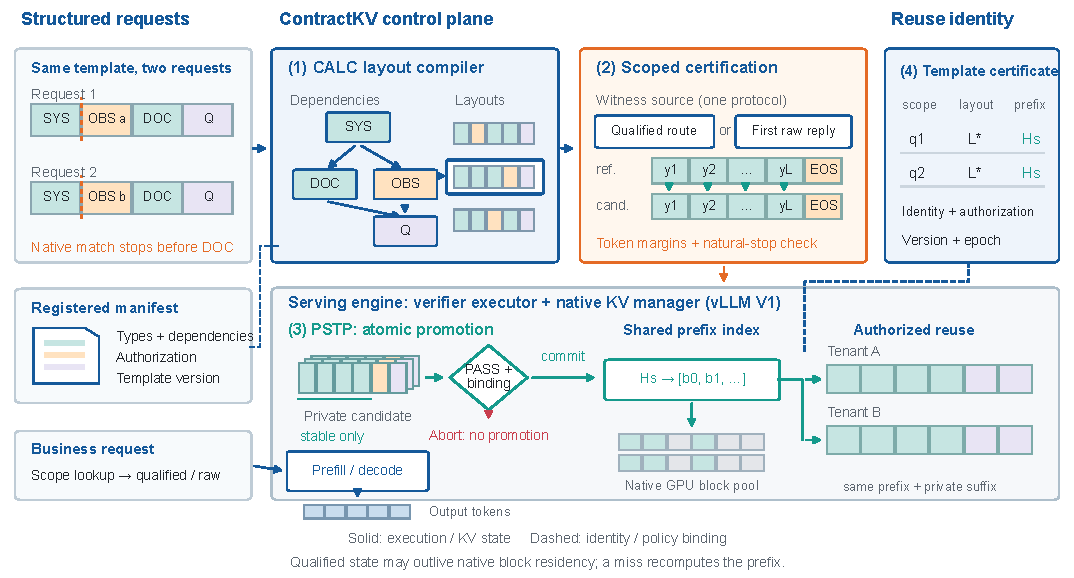
\includegraphics[width=\textwidth]{figures/fig1_architecture.pdf}
\caption{ContractKV makes a compiled stable prefix an evidence-bound service object. CALC repairs a structural prefix gap; one of two separately evaluated witness protocols supplies scoped token-path evidence; PSTP commits eligible state only after PASS and a valid binding. Authorized tenants of the same template share the prefix and keep changing suffixes private. Qualification and physical residency have separate lifetimes.}
\label{fig:architecture}
\end{figure*}

Qualification granularity is part of the service contract. We evaluate two protocols within this architecture. Deployment-qualified execution registers an already qualified template route using a representative compiled trajectory. Query-qualified execution uses the first real raw business response for each query scope as its witness, then shares the decision across authorized requests in that scope. The latter provides the stricter free-running evaluation in this paper. It requires work proportional to distinct selected query scopes, rather than one behavioral decision for arbitrary future queries. The template prefix remains a common physical reuse object across those decisions.

The primary evaluation asks whether that stricter protocol still pays for itself on preserved task inputs. Across six source-disjoint HotpotQA and RepoBench templates, three models, and three fresh-process repetitions, ContractKV achieves 1.619$\times$, 1.109$\times$, and 1.070$\times$ full-cost throughput. The service clock includes raw witnesses, failed attempts, qualification, and waiting, with zero tool slack. All 1,296 admitted compiled future pairs match their raw output IDs. Coverage and absolute task scores remain visible, and p99 increases are reported. Separate deployment experiments demonstrate qualification amortization and controlled publication; block-level probes distinguish valid qualification from the continued residency needed to realize a hit.

The paper makes four contributions, each connecting a mechanism to observable service behavior:
\begin{itemize}
\item \textbf{Contract-aware compilation} of bounded, dependency-valid layout candidates with exact rendered-token identities (Section~\ref{sec:calc}).
\item \textbf{Scoped model-backed admission} that binds token-path and termination evidence to declared inputs and execution conditions, evaluated with real free-running generation (Sections~\ref{sec:scope} and~\ref{sec:quality}).
\item \textbf{Transactional KV publication} at an exact-LCP, block-aligned commit boundary, with zero promotion for rejected candidates (Sections~\ref{sec:pstp} and~\ref{sec:ablation}).
\item \textbf{Service-template reuse} that separates behavioral decision granularity from physical prefix identity and measures amortization, full service cost, and cache availability (Sections~\ref{sec:template}, \ref{sec:mainresults}, and~\ref{sec:deployment}).
\end{itemize}
